\section{Hệ hỗ trợ quyết định: dự báo nhu cầu và lượng nhập}\label{sec:dss}
\subsection{Bài toán và lý do chọn hướng}
Với một phạm vi tùy chọn (toàn kho, một bang hoặc một danh mục), DSS trả lời hai câu hỏi là tháng tới bán được bao nhiêu và nên nhập bao nhiêu.

Hướng ban đầu là phân khúc khách hàng bằng RFM và K-Means. Nhóm đã thử trên dữ liệu thật với kiểm tra theo thời gian (huấn luyện trước, kiểm tra sau) và thấy dữ liệu không đủ thông tin về hành vi quay lại. Cụ thể, 97\% khách (90.557/93.358) chỉ mua một lần nên điểm tần suất gần như hằng số và tỷ lệ mua lại trong 180 ngày chỉ khoảng 3,1\%. K-Means và mô hình có giám sát dùng cùng đặc trưng đều dự đoán việc mua lại chỉ hơn ngẫu nhiên một chút, còn mức đánh giá (review) và việc giao trễ cũng không liên quan đến việc khách mua lại. Ngược lại, nhu cầu theo tháng có thể đo sai số bằng backtest và không cần giả định về hành vi khách, nên DSS chuyển sang dự báo nhu cầu và nhập hàng.

\subsection{Dữ liệu đầu vào}\label{sec:dss-data}
View \code{dw.v_dss_monthly_demand} (\code{sql/dss/01_demand_mart.sql}) tổng hợp đơn delivered theo tháng $\times$ bang $\times$ danh mục với ba cột: số món (\code{units}, số dòng \code{fact_sales}), doanh thu hàng (\code{revenue}) và số đơn. View chỉ đọc kho, không đổi schema và được pipeline tạo lại sau mỗi lần nạp; tổng của nó đối soát khớp với \code{fact_sales} delivered (13.221.498,11 R\$; 110.197 món). Chuỗi lịch sử bắt đầu từ 01/2017 vì đây là tháng đầu của đoạn liên tục. Trước đó, 10/2016 có 313 món nhưng 11/2016 không có đơn nào và 12/2016 chỉ có 1 món. Hai tháng gần như trống này phản ánh khoảng hở của dữ liệu chứ không phải nhu cầu thật; nếu đưa vào, chuỗi sẽ có một cú sụt về 0 rồi bật lên 913 món ở 01/2017, làm Holt học sai xu hướng và làm tăng mẫu số MASE. Hệ thống không nội suy tháng thiếu nên chọn bỏ đoạn này thay vì tự điền số; tháng cuối là tháng gần nhất có số món ít nhất 30\% trung vị các tháng, để một tháng mới nạp dở không bị coi là tháng thật. Với dữ liệu hiện có đó là 08/2018, nên tháng dự báo là 09/2018.

\subsection{Mô hình dự báo và đo sai số}
Chuỗi lịch sử chỉ có khoảng 20 điểm theo tháng nên nhóm chọn các phương pháp đơn giản, ít tham số, thay vì mô hình học máy dễ quá khớp. Bốn cách dự báo trước một tháng được so sánh: naive (lấy tháng trước, dùng làm mốc so sánh), trung bình 3 tháng, Holt có suy giảm xu hướng và kết hợp (trung bình của naive và Holt, là mặc định). Kết hợp được chọn vì naive thường lệch thấp còn Holt lệch cao, nên trung bình bù trừ độ thiên lệch.

Mô hình Holt có suy giảm xu hướng \cite{fpp} dự báo theo công thức
\begin{equation}
\hat y_{t+1}=\ell_t+\phi\, b_t,\qquad 0<\phi<1,
\end{equation}
trong đó $\ell_t$ là mức hiện tại và $b_t$ là xu hướng hiện tại, cả hai được làm mịn theo từng tháng. Nhóm chọn mô hình này vì doanh số 2017--2018 có xu hướng tăng rõ nên cần mô hình có xu hướng, đồng thời hệ số suy giảm $\phi$ làm xu hướng yếu dần theo thời gian, tránh ngoại suy thẳng một đà tăng ngắn hạn. Nói cách khác, dự báo bằng mức hiện tại cộng một phần xu hướng gần nhất; tham số làm mịn và $\phi$ được chọn bằng lưới sao cho sai số dự báo một bước trên lịch sử là nhỏ nhất.

Sai số được đo bằng backtest trượt, tức là với mỗi tháng từ tháng thứ 7 (07/2017) đến 08/2018, mô hình chỉ dùng dữ liệu trước tháng đó, nên sai số đo được mô phỏng đúng tình huống dự báo thật. Sai số được báo cáo bằng hai thước đo, mỗi thước có một lý do riêng:
\begin{align}
\mathrm{WAPE}&=\frac{\sum_t |y_t-\hat y_t|}{\sum_t y_t}\ \text{\cite{kolassa}},\\
\mathrm{MASE}&=\frac{1}{n}\sum_t \frac{|y_t-\hat y_t|}{\mathrm{MAE}^{naive}_{<t}}\ \text{\cite{hyndman}}.
\end{align}
WAPE là tổng sai số tuyệt đối chia tổng lượng bán, tức cho biết ``dự báo lệch bao nhiêu phần trăm so với lượng bán thực''. Thước đo này được chọn thay cho MAPE vì MAPE chia từng tháng riêng nên bị phóng đại ở các tháng bán thấp (ví dụ 2016 hoặc danh mục nhỏ), trong khi WAPE tính trọng số theo quy mô và phù hợp với bài toán tồn kho \cite{kolassa}. MASE chia sai số cho sai số trung bình của dự báo ``tháng trước'' trong dữ liệu đã có tại thời điểm dự báo, nên cho biết mô hình tốt hơn hay kém hơn naive bao nhiêu lần (nhỏ hơn 1 nghĩa là tốt hơn). Thước đo này được thêm vì không phụ thuộc đơn vị, nên so sánh được giữa các bang và danh mục có quy mô rất khác nhau, điều mà WAPE khó làm công bằng; mẫu số chỉ dùng dữ liệu trước tháng dự báo nên không rò rỉ thông tin tương lai \cite{hyndman}.

\subsection{Lượng nhập đề xuất}
Gọi $e_t=y_t-\hat y_t$ là sai số từng tháng backtest (dương nghĩa là cầu vượt dự báo, nguy cơ thiếu hàng). Lượng nhập tháng tới được tính bằng dự báo cộng một khoản đệm an toàn:
\begin{equation}
\text{Lượng nhập}=\max\bigl(\hat y_{\text{tháng tới}}+Q_{p}(e),\,0\bigr),
\end{equation}
với $Q_p$ là phân vị mức $p$ của các sai số $e_t$ (nội suy tuyến tính), $p\in\{85\%,90\%,95\%,99\%\}$ do người dùng chọn, mặc định 90\% \cite{trapero}. Nhóm chọn cách này vì tồn kho an toàn thường được tính bằng công thức dựa trên phân phối chuẩn của sai số, nhưng với 12--14 điểm và sai số lệch (tháng Black Friday), giả định đó không đáng tin; cách phân vị thực nghiệm không cần giả định phân phối và dùng trực tiếp những sai số đã quan sát \cite{trapero}. Ngưỡng 85--99\% là dải mức phục vụ mà bài báo này dùng. Hiểu đơn giản, đệm là mức thiếu hụt mà $p$ phần trăm số tháng quá khứ không vượt quá; đệm có thể âm nếu mô hình thường dự báo cao hơn thực tế.

Vì mẫu nhỏ, mức $p$ danh nghĩa không bảo đảm tỷ lệ không thiếu hàng thực sự. Do đó hệ thống thêm đường đánh đổi đo bằng leave-one-out. Với mỗi tháng, đệm chỉ học từ các tháng khác, lượng nhập của tháng đó là dự báo cộng đệm, rồi đếm tỷ lệ tháng thiếu hàng và mức dư hàng. Cách này được chọn vì mẫu quá ít để chia riêng một tập kiểm tra, trong khi leave-one-out vẫn dùng mọi tháng mà không để tháng nào tự học từ chính nó. Nhờ đó, người ra quyết định thấy được mỗi mức an toàn đánh đổi bằng bao nhiêu hàng dư để giảm bao nhiêu rủi ro thiếu hàng. Công tắc ``bỏ Black Friday khỏi mẫu sai số'' (mặc định bật) loại hai tháng 11--12/2017 vì tháng tới không phải tháng sự kiện.

\subsection{Backend và giao diện}
DSS có ba API là \code{/api/dss/options}, \code{/api/dss/forecast} và \code{/api/dss/accuracy}; phần tính toán nằm trong một mô-đun thuần Python có kiểm thử đơn vị. Màn Quyết định cho chọn phạm vi, thước đo (số món hoặc doanh thu), mức an toàn và cách dự báo. Đầu trang là thẻ kết luận ``Nên nhập khoảng \ldots{} món'', bên dưới là biểu đồ bán thực tế và dự báo, đường đánh đổi theo mức an toàn, sai số theo mức chi tiết và bảng so sánh các cách dự báo.

Hình~\ref{fig:ui-dss} là màn Quyết định cho toàn kho, đo bằng số món, ở mức an toàn 90\%.

\begin{figure}[H]\centering
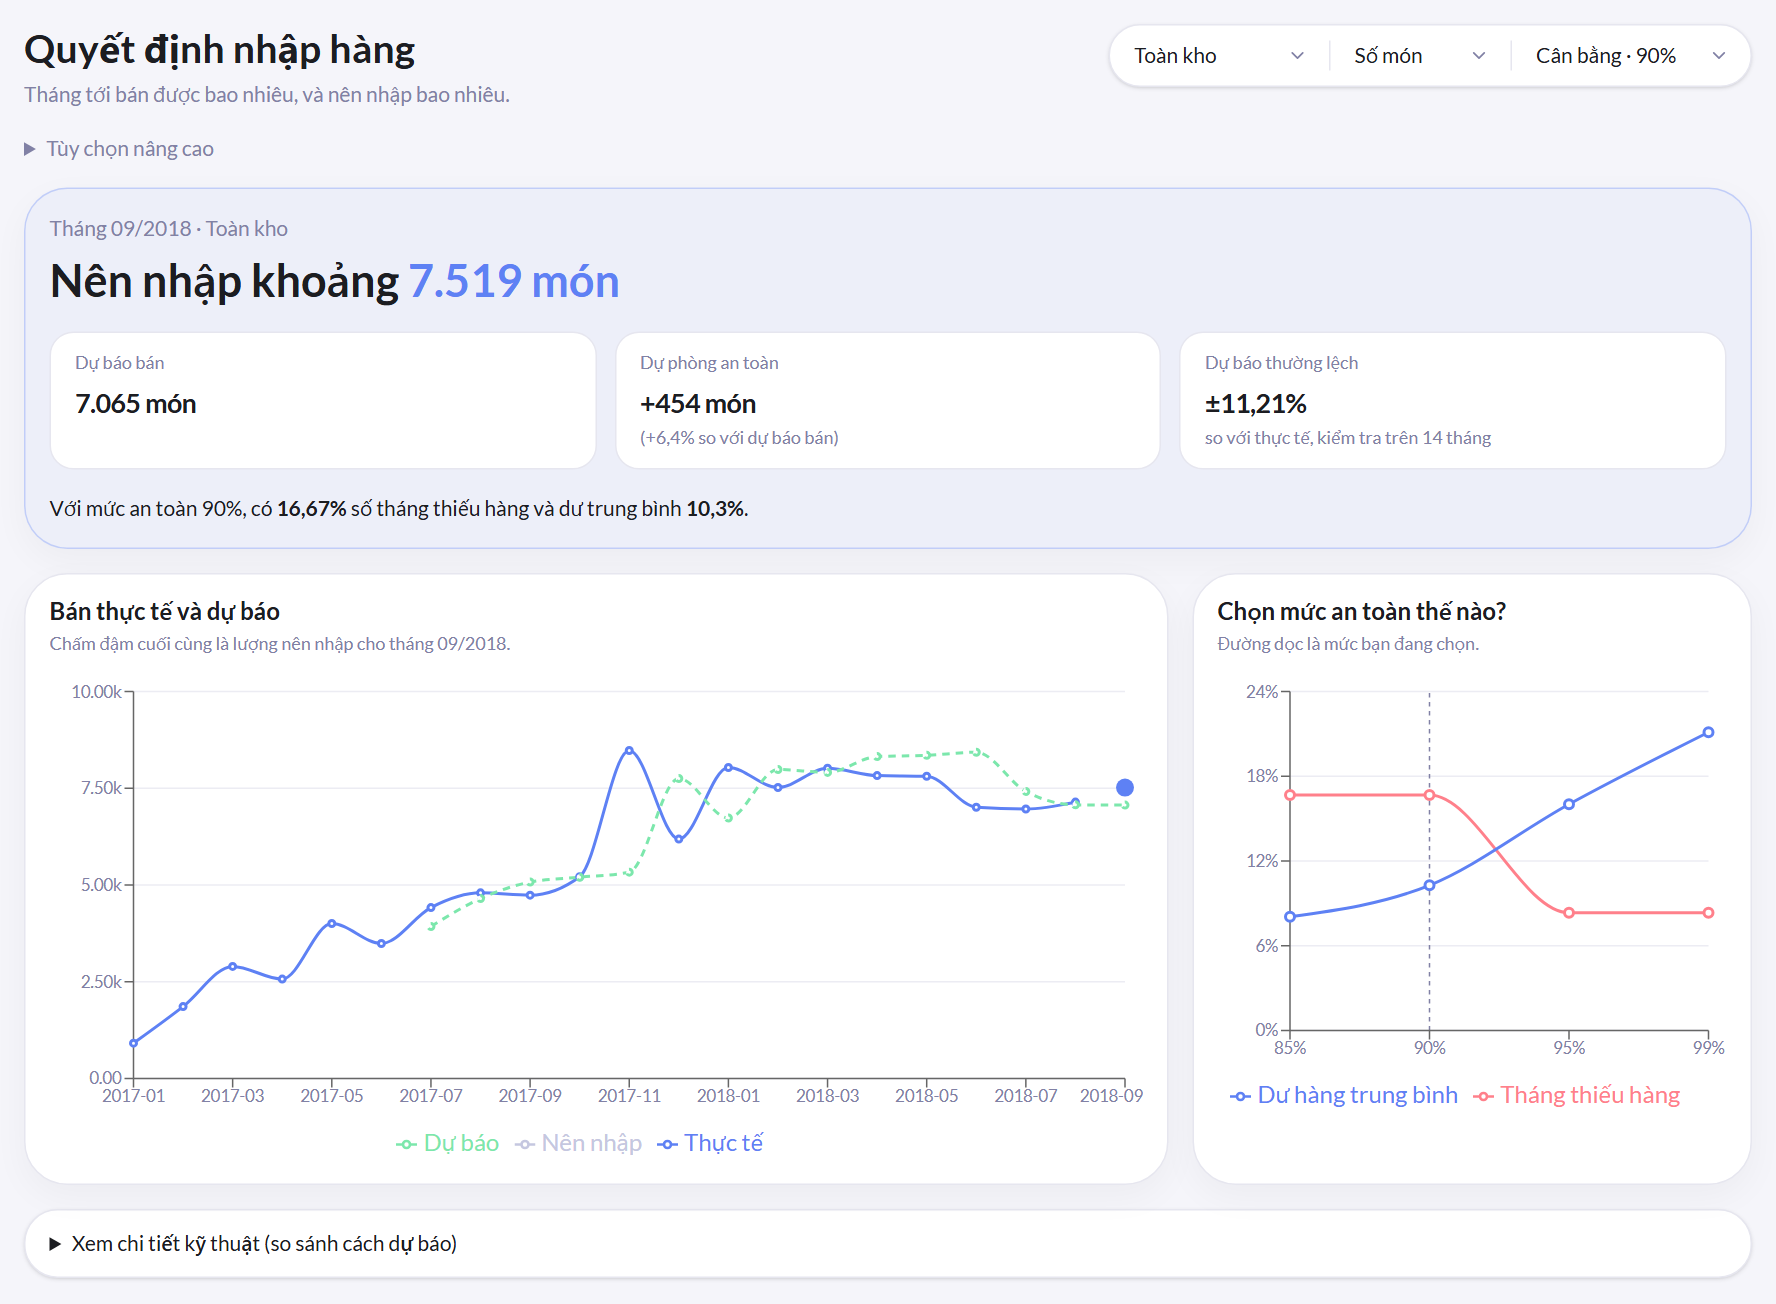
\includegraphics[width=\linewidth,height=0.5\textheight,keepaspectratio]{assets/ui_dss.png}
\caption{Màn Quyết định}\label{fig:ui-dss}
\end{figure}

\subsection{Kết quả}
\begin{table}[H]\centering\small
\begin{tabularx}{\linewidth}{Yr}
\toprule Chỉ số (toàn kho, số món, tháng dự báo 09/2018) & Giá trị\\\midrule
Dự báo bán (mô hình kết hợp) & 7.065 món\\
Đệm ở mức 90\% (bỏ Black Friday, 12 tháng trong mẫu) & +453,64 món (+6,4\%)\\
Lượng nhập đề xuất & 7.518,82 món\\
Tỷ lệ tháng thiếu hàng thực nghiệm ở mức 90\% (leave-one-out) & 16,7\% (2/12 tháng)\\
\bottomrule\end{tabularx}
\caption{Đề xuất nhập hàng toàn kho}
\end{table}

\begin{table}[H]\centering\small
\begin{tabularx}{\linewidth}{Yrrrr}
\toprule Mức tổng hợp & WAPE kết hợp & WAPE tháng trước & MASE kết hợp & MASE tháng trước\\\midrule
Toàn kho & 11,2\% & 12,2\% & 0,88 & 0,97\\
10 bang lớn & 12,9\% & 15,0\% & 1,01 & 1,12\\
15 danh mục lớn & 20,0\% & 20,7\% & 1,23 & 1,27\\
\bottomrule\end{tabularx}
\caption{Sai số backtest theo mức tổng hợp}\label{tab:dssaccuracy}
\end{table}

Mức tổng hợp càng cao càng chính xác. Mô hình kết hợp chỉ hơn mốc ``tháng trước'' một khoảng nhỏ (khi bỏ Black Friday, chênh lệch gần như biến mất, chỉ còn 7,4\% so với 7,5\% ở toàn kho); ở mức bang và danh mục chính mốc naive cũng có MASE trên 1. Có hai lý do. Thứ nhất, giai đoạn kiểm tra biến động mạnh hơn lịch sử. Thứ hai, mỗi chuỗi nhỏ hơn nhiều: theo cách đếm trên CSV với cùng cửa sổ 01/2017--08/2018, trung vị số món mỗi tháng của 10 bang lớn là 231 (từ 110 đến 2.316) và của 15 danh mục lớn là 218,5 (từ 75 đến 557,5), so với khoảng 5.700 ở toàn kho. Chuỗi càng nhỏ thì càng nhiễu, trong khi chỉ có khoảng 20 điểm để học, nên sai số tăng khi xuống mức chi tiết chủ yếu là hệ quả của dữ liệu ít chứ chưa chắc là điểm yếu riêng của mô hình, vì mốc naive cũng chịu cùng mức nhiễu. MASE được dùng để so sánh các mô hình với nhau thay vì so với mốc 1. Tham số số tháng lịch sử tối thiểu ($=6$) do nhóm tự đặt; thay đổi từ 3 đến 10 làm lượng nhập dao động khoảng $\pm 5\%$ quanh 7.500 món (7.214--7.972) và tỷ lệ thiếu hàng thực nghiệm từ 9\% đến 17\%. Vì vậy kết luận nên đọc là ``khoảng 7.500 món'' hơn là một con số chính xác.

\subsection{Hạn chế}
Dữ liệu chỉ có khoảng 20 tháng nên mẫu sai số chỉ 12--14 tháng, làm đệm nhạy với từng tháng bất thường. Tỷ lệ thiếu hàng đo được là 16,7\% (2 trên 12 tháng), cao hơn mức danh nghĩa 10\%, nhưng mỗi tháng thiếu hay không thiếu làm con số đổi khoảng 8,3 điểm phần trăm. Chênh lệch này vì vậy nằm trong mức dao động của mẫu nhỏ và chưa đủ để kết luận cách tính đệm sai; phép thử đổi số tháng lịch sử tối thiểu cũng cho tỷ lệ từ 9\% đến 17\%. Ở mức bang và danh mục, mỗi chuỗi chỉ có vài trăm món mỗi tháng nên sai số lớn hơn toàn kho. DSS chỉ dự báo trước một tháng, chưa có khoảng dự báo dạng băng trên biểu đồ và chưa xét tồn kho hiện có hay thời gian giao hàng của nhà cung cấp.
